%%%%%%%%%%%%%%%%%%%%%%%%%%%%%%%%%%%%%%%%%%%%%%%%%%%%%%%%%%%
%% Arquitectura y Modelamiento 

\section{Modelado del software.}\label{modelado:modelado-del-software}

\subsection{Arquitectura.}\label{modelado:arquitectura}
La principal decisión de diseño es construir una arquitectura que permita modificarse a lo largo del desarrollo, para ello se dividirá la funcionalidad del software en Unidades Manager. Estas unidades además de delimitar scopes, irán construyendo en conjunto un lenguaje común de funciones y variables, acorde a la lógica de funcionamiento del sistema. Es decir, el nombre de las funciones y variables de cada manager tendrán coherencia externa generando idealmente una “narración” del funcionamiento del código. De esta forma la flexibilidad de la arquitectura permitirá cambiar y generar lo que se espera de cada dominio del Manager.

Por ejemplo, tendremos la posibilidad de fusionar el manager de música con el de sonido, o separar el sistema de datos en un sistema que interactúe con una base de datos de idiomas y otro que parsee archivos de misiones, etc.

\begin{figure}[h]
	\centering
	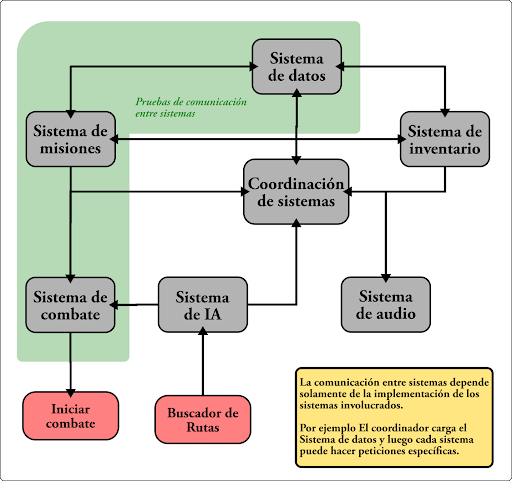
\includegraphics[width=0.6\textwidth]{imágenes/arquitectura.png}
	\caption{Ejemplo de arquitectura ajustable.}
\end{figure}

\Needspace{2\baselineskip}
El enfoque agrupa los distintos comportamientos esperados a nivel de funciones al tiempo que favorece el surgimiento de una narrativa en cuanto a los nombres de las clases, funciones, variables y su sentido dentro del sistema global. Se trata de generar una especie de cadena de producción que opera en base a inputs y outputs esperados.

Por último e igual de relevante, esta encapsulación de funcionalidad va a servir para enfocar de mejor manera los distintos test unitarios que se generen en el desarrollo. Esto incluso permite agrupar una serie de comportamientos esperados, para generar objetos y variables de casos o situaciones específicas, con el fin de comprobar interacciones entre los distintos Managers (test de interacción).

En cuanto a su implementación, quizás el mayor desafío sea que la interacción con el modelo de Godot no lastre el rendimiento.

\subsection{Sistema de Managers.}\label{modelado:sistema-de-managers}
\subsection*{\noindent\normalfont\textit{Enfoque de diseño a priori.}}

Como adelantamos, la idea principal es desacoplar los distintos niveles lógico-funcionales del diseño, de la implementación de los niveles y el resto del contenido.

Este sistema de managers por tanto, vendrá a funcionar como una especie de motor lógico dentro de la implementación en Godot. Para ello, se encapsularán las distintas áreas del juego en una serie de submanagers (o cajas negras) y un manager principal que los coordine llamado GameManager (\lsc{GM}).

\pagebreak[4]
\begin{center}
	\color{colortableborder}
	\setlength{\arrayrulewidth}{1pt} 
	\rowcolors{1}{colortablebg}{colortablebg}
	\begin{longtable}{|p{0.2\linewidth}|p{0.725\linewidth}|}
		\hline
		\endhead
		\rowcolor{colorthbg}\multicolumn{2}{|l|}{\color{colorthtext}\textbf{GameManager}} \\
		\hline
		\multicolumn{2}{|p{0.961\linewidth}|}{\color{colortextotabla}Manager principal a nivel de ejecución cuya función además de iniciar el juego será la de instanciar al resto de SubManagers. \lsc{GM} tendrá una clara tendencia a crecer en complejidad por lo que es muy importante que opere delegando funciones más que implementándolas. En esta misma línea si la interacción entre managers termina siendo demasiado compleja entonces será un síntoma de que es necesario un rediseño en cuanto a los in/outs de los submanagers implicados.} \\
		\hline
		\rowcolor{colorthbg}\color{colorthtext}\textbf{SubManager} & \color{colorthtext}\textbf{Dimensión} \\
		\hline
		\color{colorthalt}LevelManager & \color{colortextotabla}Todo lo relativo a los niveles. Por ejemplo el conjunto de métodos que se encargan de toda la lógica relevante del nivel, una interfaz para que \lsc{GM} pueda conectar los distintos requerimientos del nivel, carga de locaciones, ubicación e inicio de subrutinas de Player y \lsc{NPC}, señales de áreas para CutsceneManager, \lsc{UI} específicas, etc. 
		Al igual que \lsc{GM} posiblemente tenderá a complejizarse por lo que es importante estar pendiente de posibles desacoplamientos. \\
		\hline
		\color{colorthalt}QuestManager & \color{colortextotabla}Todo lo relevante a las misiones: requerimientos, objetivos, experiencia, ítems, cutscenes, niveles, etc. \\
		\hline
		\color{colorthalt}Cutscene\newline{}Manager & \color{colortextotabla}Todo lo relativo a los momentos en el que el jugador no está interactuando con la \lsc{UI} ni tiene control del personaje, es decir animaciones dentro y fuera del gameplay. Incluye diálogos pero estudiar si es conveniente una separación. \\
		\hline
		\color{colorthalt}PlayerManager & \color{colortextotabla}Todo lo relativo al jugador: estados, ítems, exp, estadísticas, estados de misiones, controles, path del árbol de decisiones, etc. Implementar una state machine.\\
		\hline
		\color{colorthalt}IAManager & \color{colortextotabla}Todo lo referente a IA: Rutas de \lsc{NPC}, combate de \lsc{NPC} aliados y enemigos y si compete, la generación procedural de niveles. \\
		\hline
		\color{colorthalt}UIManager & \color{colortextotabla}Todo lo relativo a la interfaz gráfica: Barras de vida, visualización del mapa, menús, inventario, árbol de habilidades e interfaz de diálogo. \\
		\hline
		\color{colorthalt}AudioManager & \color{colortextotabla}Control de la música, transiciones, volumen, etc.; y los sonidos de los distintos objetos, su paneo, volumen, efectos, etc. \\
		\hline
		\color{colorthalt}Debug\newline{}Manager & \color{colortextotabla}Interfaz de debug que obtenga información relevante para el desarrollo sobre el funcionamiento de los distintos managers y objetos instanciados. \\
		\hline
	\end{longtable}
\end{center}

\subsection{Diagrama del sistema de managers.}\label{modelado:diagrama-del-sistema}
\todoii{ToDo: Hacer diagrama}{Hacer diagrama de managers}

\subsection{Funcionamiento general.}\label{modelado:funcionamiento-general}
Al partir, lo primero es iniciar GameManager que instancia los submanagers correspondientes para mostrar las escenas de presentación y luego iniciar el menú principal del juego. La escena del menú principal enviará señales a \lsc{GM} para que se inicie una nueva partida, se cargue o continúe partidas guardadas, se ajusten opciones, se inicien actualizaciones o se cierre el juego.

Independiente del sistema o mecanismo para iniciar o cargar una partida, será LevelManager el encargado cargar y conectar la lógica del nivel; esto es cargar el mapa, los sprites, scripts de cutscenes, instanciar objetos, cargar música y sonidos ambiente, asignar quests activas, etc. Es LevelManager quien lee la información o scripts de un nivel concreto e informa a \lsc{GM} para conectar estas señales con los submanagers correspondientes.

A continuación una idea preliminar general o una guía a la implementación de los distintos managers:

\subsubsection{GameManager.}\label{modelado:gamemanager}

\begin{description}%[style=unboxed] % unboxed falla al exportar a html
	\item[Descripción:] Encargado de coordinar los submanagers e iniciar y controlar las distintas funciones de ejecución del programa (incluye la velocidad del juego).
	
	\item[Consideraciones:] \lsc{GM} tendrá tendencia o a crecer o delegar en exceso, volviéndose inútil. La idea es que cuando un submanager necesite datos o funciones de otro submanager sea \lsc{GM} quien llame la función y no el propio submanager. De esta forma estaremos respetando la encapsulación del diseño y flexibilizando el código ya que en caso de desacoplar funciones de un submanager, no romperíamos la interacción entre sistemas y solo será necesario ajustar la llamada en \lsc{GM}.
	
	\item[Funcionamiento:] Colección de métodos que accedan a data de los submanagers, cambien sus estados y/o informen de ellos. Controlar los estados del juego.
\end{description}
	
\subsubsection{LevelManager.}\label{modelado:levelmanager}
\begin{description}
	\item[Descripción:]	Carga las escenas \lsc{TSCN} de los niveles y su lógica. Envía señales o ejecuta métodos para conectar las señales del nivel entre submanagers.
	
	\item[Consideraciones:] También va a tender a crecer en complejidad, por lo mismo es importante delegar funciones específicas a los submanagers correspondientes y estar atentos a posibles rediseños en cuanto a su encapsulación.
	
	\item[Funcionamiento:] Carga y almacena los niveles. Contiene funciones del tipo load\_level(level). El objeto level podría contener el mapa, música, áreas interactivas y objetos del nivel como props, \lsc{NPC} y player. La idea es que el sistema procese automáticamente todos los elementos relacionados al nivel.
\end{description}
	
\subsubsection{QuestManager.}\label{modelado:questmanager}
\begin{description}
	\item[Descripción:] Controla el flujo de las quest en el gameplay, contiene los estados de las quests activas y actualiza el árbol de decisiones del jugador. Carga los distintos objetos o elementos de la quest en el o los niveles que corresponda. Dentro de estos elementos encontramos por ejemplo opciones de diálogo, ítems, áreas de interacción, \lsc{NPC}, etc.
	
	\item[Consideraciones:] Cada quest es inicialmente un archivo de hoja de cálculo con todos los detalles de la quest que pasará por una herramienta del kit de desarrollo (apartado \nameref{i18n:toolkit-y-api}) para importarse dentro de Godot como un nodo Quest o similar. La idea es que QuestManager sea capaz de interpretar estos nodos en tiempo de ejecución para simplificar los procesos de testeo y diseño. Es importante recordar que todos los métodos que trabajen con texto deben ajustarse a los métodos de l10n pertinentes (ver el apartado \nameref{i18n:implementacion}).
	
	\item[Funcionamiento:] Extraer la data de los archivos quest referenciados por el nivel e incorporarlos al runtime del juego. Se debe mantener un control de las decisiones del jugador con respecto a las quests ya finalizadas y las que se encuentran en curso para modificar tanto quests, como diálogos disponibles según el árbol de decisiones u otras decisiones narrativas. El objeto Quest idealmente debería contener solo data y getter/setters.
	Sobre cómo se adjunta el objeto Quest a la colección de Quest activas, puede ser un comando específico en CutsceneManager o un objeto “interactible” que se adose a un área, un ítem, a una opción del diálogo, etc.
\end{description}
	
\subsubsection{CutsceneManager.}\label{modelado:cutscenemanager}
\begin{description}
	\item[Descripción:] Controla los momentos del juego en que el jugador no tiene el manejo directo de algún personaje o interfaz; se incluyen también los diálogos entre los \lsc{NPC} y/o el jugador. Cada cutscene corresponderá a un archivo de guión procesado por la herramienta del toolkit que la convertirá desde un formato de planilla de datos a un nodo dentro de Godot. Este nodo contendrá un listado de acciones secuenciales y la información requerida para su ejecución; será trabajo de CutsceneManager implementarlas y ejecutarlas. Las acciones van desde transiciones, fades a negro, diálogos, efectos atmosféricos, efectos de sonido, dar o quitar objetos; a mover \lsc{NPC}, agregar quests, cambios de estados de props, aparición de enemigos, etc.
	
	\item[Consideraciones:] Lo principal es implementar un sistema de scripts que interprete las distintas instrucciones para los guiones adjuntos. La idea es que todas estas instrucciones se puedan ajustar directamente desde el archivo (o Godot). Dado que trabajará con texto, no olvidar hacer los ajustes necesarios para la l10n del contenido (ver el apartado \nameref{i18n:implementacion}).
	
	\item[Funcionamiento:] Cada nodo cutscene podría adjuntarse a un área de activación/interacción, a una entrada de diálogo, al tomar o activar un ítem, según condiciones de tiempo, quest completadas, etc. Al activarse la cutscene, CutsceneManager va interpretando y ejecutando las distintas líneas del guión según corresponda. Por ejemplo para los diálogos, cada línea podría tener una primera columna para identificar al personaje hablante, luego la siguiente que señale qué sprite usar (quizás asociado a alguna emoción del tipo enojo, alegría, herido, etc.).
	
	Como se comentó en QuestManager, quizás sea útil un objeto “Interactible” que se pueda anexar a objetos relevantes como a un área de interacción, un timer, una transición, una opción de diálogo, etc.
\end{description}
	
\subsubsection{PlayerManager.}\label{modelado:playermanager}
\begin{description}
	\item[Descripción:] Encargado de la conexión entre el objeto Player con el resto del sistema. Controla o informa los cambios en los estados de la \lsc{FSM} (Finite State Machine) del jugador, además de contener los distintos stats tales como experiencia, nivel, equipamiento, items de quest, munición, etc. Además, contiene el árbol de decisiones de quests y diálogos clave.
	
	\item[Consideraciones:] Por el propio diseño que propone Godot, quizás mucha de estas funciones terminen siendo implementadas en la escena Player, sobre todo lo referente a la \lsc{FSM}. Para que el acoplamiento de ese código tenga un scope y relación coherente con los otros managers, es esencial estudiar la forma en que PlayerManager y la escena Player terminan interactuando entre sí y desde PlayerManager a \lsc{GM} y al resto del sistema.
	
	Quizás mucha de la funcionalidad descrita termine siendo implementada en la escena Player en Godot sobre todo lo referente a la \lsc{FSM}. En ese sentido para que ese acoplamiento de código tenga un scope e interacción coherentes con el sistema, es esencial estudiar la forma en que PlayerManager y la escena Player terminan interactuando entre sí y con el resto de managers.
	
	\item[Funcionamiento:] La escena Player podría tener nodos de sprite, \lsc{FSM} (con estados anexables), controles, animaciones, data y todo lo que interactúe directamente con los elementos visuales del juego. Por su parte PlayerManager debería controlar todo lo referente a la lógica del sistema de juego, vale decir los stats, modificadores de equipamiento al ataque, velocidad, árbol de decisiones, etc.
\end{description}
	
\subsubsection{IAManager.}\label{modelado:iamanager}
\begin{description}
	\item[Descripción:] Encargado de conectar los métodos de IA con los distintos funcionamientos del juego, es decir los sistemas de inteligencia artificial de los enemigos en combate, el sistema de tácticas de aliados, pathfinding de \lsc{NPC} y si compete un generador de niveles procedural. 
	
	\item[Consideraciones:] Probablemente sea la dimensión más difícil de implementar, por lo mismo se propone no comenzar de inmediato con el código sino investigar las distintas tecnologías disponibles y estudiar su implementación en Godot y dentro del sistema de managers del juego. Además debido a esta complejidad, lo más probable es que sea necesario utilizar un lenguaje de más bajo nivel como C\texttt{++} para mantener una buena performance del sistema. Considerar la la división a submanagers más específicos.
	
	\item[Funcionamiento:] Define en tiempo real las rutas de movimiento de los \lsc{NPC}, además de estrategias de ataque y posicionamiento tanto de enemigos como aliados en combate. Genera niveles en base a heurísticas de acoplamiento y optimización.
\end{description}
	
\subsubsection{UIManager.}\label{modelado:uimanager}
	\begin{description}
	\item[Descripción:] Controla toda la interfaz gráfica del juego y sus elementos como \lsc{HUD}, pantallas de inventario, equipamiento, menús del juego, escenas de diálogo, burbujas de texto, ayudas, letreros, mapas, información de debug, etc.
	
	\item[Consideraciones:] Idealmente debe proveer una interfaz para que la información en la pantalla de los distintos managers se actualice cuando corresponda. Debe resolver un modo debug que muestre toda la información relevante al desarrollo. Si compete, se puede delegar esta funcionalidad a un DebugManager.
	
	\item[Funcionamiento:] Colección de escenas Godot que se muestran en función del estado del juego. Estas escenas envían señales a través de UIManager.
\end{description}
	
\subsubsection{AudioManager.}\label{modelado:audiomanager}
\begin{description}
	\item[Descripción:] Encargado de manejar todos los sonidos del juego incluyendo música y efectos. Debe controlar los efectos de sonidos (por ejemplo reverb en cuevas), paneos (por ejemplo en base a la posición en pantalla) y los fundidos entre canciones.
	
	\item[Consideraciones:] Tratar que los distintos parámetros (duración de transiciones, ganancia, etc.) se puedan ajustar directamente desde la interfaz de Godot.
	
	\item[Funcionamiento:] Quizás utilizar las animaciones de Godot para las transiciones. Los eventos deberían enviar archivos de audio y parámetros.
\end{description}
	
\subsubsection{DebugManager.}\label{modelado:debugmanager}
\begin{description}
	\item[Descripción:] Permite observar los diferentes estados de los distintos objetos de la ejecución, en especial aquellos relevantes para el control de flujo.
	
	\item[Consideraciones:] Idealmente debe ser independiente al funcionamiento del juego y no debería intervenir directamente los distintos managers sino ocupar los IO disponibles de cada uno y no generar código específico dentro de los managers para debug.
	
	\item[Funcionamiento:] Nodo adosable al objeto que queremos debuggear y que imprima en la consola de Godot o directamente en la pantalla la información relevante. Quizás algo parecido a la consola en algunos juegos tipo Fallout o Quake.
\end{description}

\subsubsection{Otros managers.}\label{modelado:otros-managers}
Como se ha comentado, quizás sea necesario agregar otros managers más específicos como por ejemplo InventoryManager, ItemsManager, DialogueManager, SaveManager, etc. Lo principal es mantener la coherencia del sistema y mantener un diseño limpio.

\subsection{Otras consideraciones.}\label{modelado:managers-otras-consideraciones}
\subsubsection{Plantillas.}
Algunos managers utilizarán objetos estandarizados, por ejemplo QuestManager utilizará objetos Quest, CutscenesManager Cutscenes, AudioManager Music y Audio, LevelManager objetos Level, etc. La idea es generar plantillas de estos objetos para una expedita generación de contenido.